% Benchmarking in Unity
% https://blogs.unity3d.com/2018/09/25/performance-benchmarking-in-unity-how-to-get-started/
% Maybe try VRWorks https://developer.nvidia.com/vrworks

% Questions to answer in the evaluation chapter:
% \begin{enumerate}
%   \item{How big can the graph be so that it is comfortable visualizing the network?}\\
%   What is comfortable? Number of FPS?
%   How can we scale the graph? By adding nodes and spread them around, by adding more interconnexions?
%   Should the experiment split in several parts? Scaling, filtering, moving around, etc.
%   What is the performance by using Oculus Link and the performance using just the Quest hardware?
%   -We can use the Unity GPU Profiler for Oculus Quest and Go in order to see the performance.\\
%   \href{https://developer.oculus.com/blog/getting-started-w-the-unity-gpu-profiler-for-oculus-quest-and-go/}{See: Getting Started w/ The Unity GPU Profiler for Oculus Quest and Go}
%   \item{How is this way of visualizing the graph better by using VR?}\\
%   We are researchging the technology and the test with actual users is for future work.
%   \item{In what way can the application and the visualization of the graph be improved?}\\
%   Argue in the discussion part.
% \end{enumerate}

% Links
% Profiler panel

BigNet VR has been built to explore biological networks that contain genetic information from human beings. We have used two datasets from MIxT where we applied several VR techniques to build a visualization system. In this chapter we want to evaluate this system focusing on scalability and performance problems. Since we are visualizing networks with genetic information using VR, we want to know if the system that we built can be used for any size of this type of network. As part of the evaluation process, we designed a list of questions that we will try to answer along this chapter. The questions are:
\begin{enumerate}
  \item For which interactions do we achieve the recommended FPS (72) when scaling the network?
  \item What characteristics of the network influence the scalability?
  \item What is the performance by using Oculus Link and the performance using just the Quest hardware?
  % \item Bonus: how will “beautifications” influence scalability?
  \item How do users perceive the interaction of the network?
\end{enumerate}

Question one is based on the Oculus' performance guidelines\cite{oculus_performance_baselines}, that say that an application should meet the following.
\begin{itemize}
  \item 72 FPS for Oculus Quest (required by Oculus).
  \item 50-100 draw calls per frame.
  \item 50,000-100,000 triangles or vertices per frame.
\end{itemize}

As for the second question, we want to know what characteristics influence the scalability of the system. Some parts will have more impact in the performance than others. To keep it simple, we will evaluate the impact in the performance done by the following elements, that are the most important for the visualization: number of nodes, number of lines and number of clusters.

We will also evaluate the performance of the application being run in the Oculus Quest hardware and also in a PC, using the Oculus Link cable that connects the headset to the machine. The hardware of the Oculus Quest is not as powerful as the one of the machine that was used for the development. We would like to know if the performance is good in both the machine and the headset.

Finally, as the last question says, we want to know how the users perceive the interaction and visualization of the network. We will evaluate this with a qualitative method with a demo of the application using the MIxT datasets and also an interview.

\section{Experimentation plan}
% @TODO Write about the specs of the system being used for the evaluation: the machine, software, etc.
An experimentation plan was designed to ensure that the experiments are consistent and that they can be repeated several times getting realistic measurements. We take into consideration the following aspects for our experiments:
\begin{enumerate}
  \item Scalability for different interactions.
  \item Network characteristics.
  \item Bottlenecks.
  \item User study.
  \item Hardware and software specification.
\end{enumerate}

There are some elements of the network that influence more in the scalability and performance of the system. In Table /ref{tab:network-elements} we describe these elements.

\begin{table}[h!]
\centering
\begin{tabular}{|p{4cm}|p{6cm}|}
\hline
\textbf{Element} & \textbf{Description} \\
Clusters & description for clusters \\
Nodes   & Represented as 2D squares in the space. The position is calculated when creating the clusters.  \\
Lines & They represent relationships between the nodes. Everytime a node is selected, line objects are added to the scene. \\
\hline
\end{tabular}
\caption{Elements of the network that have influence in the scalability.}
\label{tab:network-elements}
\end{table}

We ran the experiments in a machine with Windows 10. In Table \ref{tab:machine-specs} we can see some of the hardware specification from the machine used:
\begin{table}[h!]
\centering
\begin{tabular}{ll}
\multicolumn{2}{c}{Machine specification}                        \\
Processor   & Intel(R) Xeon(R) CPU E3-1275 v6 @ 2.80GHz 3.79 GHz \\
RAM memory  & 64.0 GB                                            \\
System type & 64-bit Operating System
\end{tabular}
\caption{Machine specification.}
\label{tab:machine-specs}
\end{table}

Since the GPU is important in this type of applications, we show the specs of the GPU used in Table \ref{tab:gpu-specs}.

\begin{table}[h!]
\centering
\begin{tabular}{ll}
\multicolumn{2}{c}{GPU specification} \\
Adapter type   & NVIDIA GeForce GTX 1080 Ti \\
Chip Type  &  GeForce GTX 1080 Ti \\
DAC Type & Integrated RAMDAC \\
Available memory & 45025 MB
\end{tabular}
\caption{GPU specification.}
\label{tab:gpu-specs}
\end{table}

As for the VR headset hardware, we used a Oculus Quest. In Table \ref{tab:oculus-specs} we can see the hardware specifications for this type of headset.

\begin{table}[h!]
\centering
\begin{tabular}{ll}
\multicolumn{2}{c}{Oculus Quest specifications} \\
Panel Type   & Dual OLED 1600x1440 \\
Supported Refresh Rate  &  72Hz \\
Tracking & Inside out, 6DOF \\
CPU & Qualcomm® Snapdragon 835 \\
GPU & Qualcomm® Adreno™ 540 GPU \\
Memory & 4GB total
\end{tabular}
\caption{Oculus Quest specifications.}
\label{tab:oculus-specs}
\end{table}

The experiments were run in Unity, the same software that was used for the development. The version of Unity used for the expriments is 2018.4.10f1. Also Vulkan is used as the graphic API.

% @TODO Write about how scalability was tested.
A test scene was built in order to test the network and the scalability of it. A random network is built and we test how comfortable it is to navigate through it. This is measured by the FPS rate.

VR profiling is a technique used to get an overview of the performance of our application. This is usually done in order to find bottlenecks so that we can eliminate them and improve the application's performance.

To profile the application we used the built-in profiler in Unity, the software used for the development. The Unity Profiler gives information about per-fram CPU and GPU performance metrics.

\section{Performance and scalability of the system}

We have run some experiments where we analyse the scalability of the system. We decided to analyse the parts of the system that can have more impact in the scalability and that are most used by the user when exploring the networks. These are: moving the network, scaling the network and node selection (which also includes the cration of relationships in the scene).

I will describe now the experiments that I want to run to evaluate this. The experiments will be divided in two parts. The first part consists of several experiments where I analyze the performance for each of the actions that I will focus on. The second part will focus on analyzing the scalability for the line creation, which can create bottlenecks, according to the performance analysis done.

\subsection{First part: performance}

In the first set of experiments, we are going to use the profiler from Unity, where we can see a frame chart that contains information about performance data over time on a frame-by-frame basis\footnote{https://docs.unity3d.com/Manual/ProfilerWindow.html}. We will use the blood dataset from MIxT for these experiments and we will manipulate the size of it for each of the actions that we want to evaluate: one version with a third of the nodes from the dataset, one with half of the nodes and then a final one with all the nodes. We will also remove the relationships for the nodes that doesn't exist anymore from the reduced datasets. In total we will run 9 experiments (3x3). This will produce a total of 9 screenshots that I could have as anexus (A page can contain 3 of these screenshots, each page for a different action). Furthermore I will resume the data in 3 tables like Table \ref{tab:experiment_moving}, Table \ref{tab:experiment_scale} and Table \ref{tab:experiment_select}. Each table shows the data from the experiments for a specific action. The last column shows the average of the 25\% of the worst times (so the 25\% of the frames that have higher values). An alternative to the tables could be a bar graph.

As for how I will run the experiments, I want to create a script for each action. I want to create a script that moves the network, another script that scales up and down the network and a third one that selects a few nodes. We can select the 100 first frames an run the calculations for the percentages. This can be a tedious task if I have to do it manually, it would be better if I can do it programmatically (which I haven't seen a solution for so far).

\begin{table}[h!]
\centering
\begin{tabular}{lll}
\multicolumn{2}{c}{Experiment: moving the network} \\
Number of nodes & 0.25\% average low (ms) & 0.1\% average low (ms) \\
size/3 & 11.59 & sth \\
size/2 & sth & sth \\
size & sth & sth \\
\end{tabular}
\caption{Experiment: moving the network.}
\label{tab:experiment_moving}
\end{table}

\begin{table}[h!]
\centering
\begin{tabular}{lll}
\multicolumn{2}{c}{Experiment: scale the network} \\
Number of nodes & 0.25\% average low (ms) & 0.25\% average low (ms)  \\
size/3 & 11.76 & sth \\
size/2 & sth & sth \\
size & sth & sth \\
\end{tabular}
\caption{Experiment: scale the network.}
\label{tab:experiment_scale}
\end{table}

The blood dataset has a total of 2693 nodes. Each node can have between 10 and thousands of edges with other nodes. The node with the name ARGLU1 has the highest number of edges, a total of 16070. In Figure \ref{fig:edges_nodes_blood} we show a scatter plot where the X axis represents the the number of edges in ascendent order and the Y axis represents the number of nodes that have that number of edges. As we can see, most of the nodes have less than 200 edges. But a few ones have several thousands. We have selected a few nodes for the experiments that cover nodes with lower number of edges to higher number of edges.
The nodes are: TGFBR3 (10), EPSTI1(110), SMNDC1(900), HNRNPH3(2900), ANGEL2(5860), FOPNL(11450), ACTR6(7560), ARGLU1(16070).

% Example scatter plot https://timodenk.com/blog/latex-plot-snippets/screen-shot-2017-02-18-at-15-10-07/
% https://tex.stackexchange.com/questions/390161/drawing-3d-points-from-external-file
\begin{figure}[h!]
  \centering
  \begin{minipage}{.7\textwidth}
  \begin{tikzpicture}
    \begin{axis}
    [ xlabel=Number of edges,
    ylabel=Number of nodes,
    xmin=0,xmax=16100,
    ymin=0,ymax=240,
    ]
    \addplot[scatter, only marks] file{data/bloodScatter.dat};
    \end{axis}

    \end{tikzpicture}
  \end{minipage}
\caption{Scatter plot showing a distribution of the number of edges in the blood dataset.}
\label{fig:edges_nodes_blood}
\end{figure}

\begin{table}[h!]
\centering
\begin{tabular}{lll}
\multicolumn{2}{c}{Experiment: select node} \\
Number of nodes & 0.25\% average low (ms) & 0.25\% average low (ms) \\
size/3 & 17.64 & sth \\
size/2 & sth & sth \\
size & sth & sth \\
\end{tabular}
\caption{Experiment: select node and draw lines.}
\label{tab:experiment_select}
\end{table}

\subsection{Second part: scalability}

Once we see that the selecion of the nodes (including drawing the lines) has more impact in the performance and that it can create bottlenecks, we can evaluate the scalability of the line drawing. For this I can create an experiment where I measure the time that it takes to draw the lines for the selection of 15 nodes (20 can be too many for the graph). I can do three versions of this experiment where I scale the number of relationships by 2 and 3 times. I can also show the number of lines that are drawn for each node.

I can create a linear graph for this, like the one I showed (See Figure \ref{fig:graph_scalability}). I would also like to show the number of lines that each node renders. Maybe I can show this in the x axis. Any suggestion?

Example graph:
\begin{figure}[h]
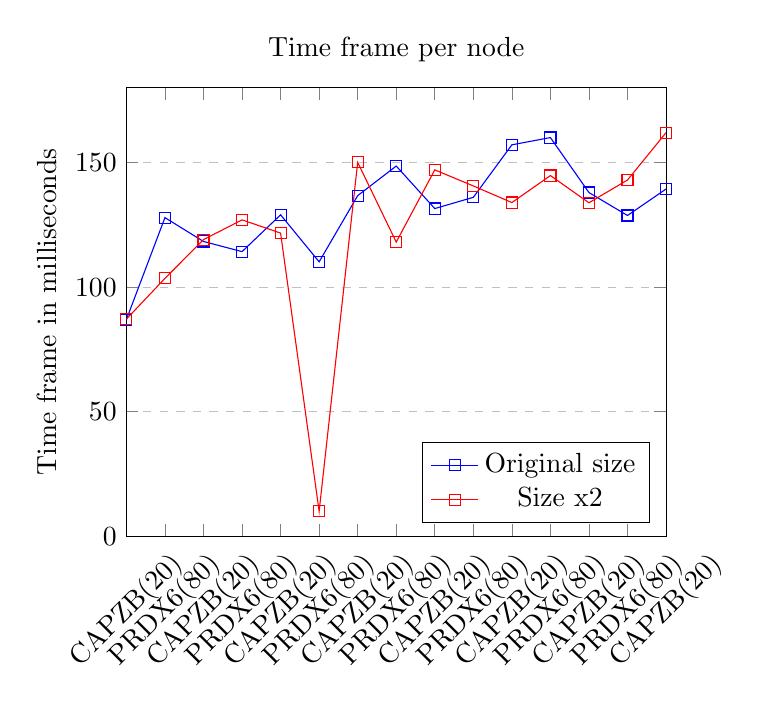
\begin{tikzpicture}
\begin{axis}[
    title={Time frame per node},
    ylabel={Time frame in milliseconds},
    xmin=1, xmax=15,
    ymin=0, ymax=180,
    xticklabel style={rotate=45},
    xtick={1, 2, 3, 4, 5, 6, 7, 8, 9, 10, 11, 12, 13, 14, 15},
    xticklabels={CAPZB(20),PRDX6(80),CAPZB(20),PRDX6(80),CAPZB(20),PRDX6(80),CAPZB(20),PRDX6(80),CAPZB(20),PRDX6(80),CAPZB(20),PRDX6(80),CAPZB(20),PRDX6(80),CAPZB(20)},
    ytick={0, 50, 100, 150, 200},
    legend pos=south east,
    ymajorgrids=true,
    grid style=dashed,
]

\addplot[
    color=blue,
    mark=square,
    ]
    coordinates {
     (1, 86.98678) (2, 127.9083) (3, 118.3348) (4, 114.2518) (5, 129.0339) (6, 110.1637) (7, 136.7278) (8, 148.6127) (9, 131.5426) (10, 136.0563) (11, 157.1314) (12, 160.0461) (13, 137.9729) (14, 128.7614) (15, 139.3922)
    };
    \addlegendentry{Original size}

\addplot[
    color=red,
    mark=square,
    ]
    coordinates {
     (1, 87.14521) (2, 103.5218) (3, 119.0831) (4, 127.0019) (5, 121.6989) (6, 10) (7, 150.0758) (8, 118.0902) (9, 147.074) (10, 140.6292) (11, 133.9567) (12, 144.7911) (13, 133.8688) (14, 143.0063) (15, 162.0063)
    };
    \addlegendentry{Size x2}

\end{axis}

\end{tikzpicture}

\caption{Data showing the scalability.}
\label{fig:graph_scalability}
\end{figure}

\section{Demo and interview}
One of the questions that we asked ourselves during the evaluation process was about the comfortability of using BigNext VR to explore a biological network. This is an important aspect when building VR applications. Some of the aspects to take into account are for instance the motion sickness or the intuitiveness. In order to evaluate this we made a questionnaire for bioinformaticians that would test the application. Unfortunately, due to the Covid-19 situtation\cite{covid_19}, we were not able to carry out the questionnaire with people. The reason is because it wasn't possible to test BigNet VR with people on a single Oculus Quest device without avoiding the social distancing rules.
We estimated to have around 10 participants with knowdledge in bioinformatics to test the application. With this number of participants we could have made some statistics and obtained feedback for future improvement.

The following questionnaire is divided in four sections; a general section about VR headsets, a section about comfortability exploring the network using BigNet VR, a section about the different actions in BigNet VR and finally a section about feedback.

To complete the questionnaire, the teste has to indicate the level of agreement or disagreement with each of the  statements, mark yes or no when it is asked and in the feedback section reply the questions with constructive feedback if possible.\\

% TODO Interview questions

% Questionnaire section 1: VR headsets.
% \begin{enumerate}
%   \item Have you ever used a VR headset before?\\
%   Yes / No
%
%   \item Have you ever used a Oculus Quest headset before?\\
%   Yes / No
%
%   \item I feel comfortable using a VR headset.\\
%   Strongly agree / Agree / Neutral / Disagree / Strongly Disagree
%
%   \item I feel comfortable using the Oculus Quest headset.\\
%   Strongly agree / Agree / Neutral / Disagree / Strongly Disagree\\
% \end{enumerate}
%
% Questionnaire section 2: Comfortability exploring a biological network with BigNet VR.
% \begin{enumerate}
%   \item I feel comfortable moving around the virtual environment using the teleport functionality.\\
%   Strongly agree / Agree / Neutral / Disagree / Strongly Disagree
%
%   \item I feel comfortable rotating to any direction.\\
%   Strongly agree / Agree / Neutral / Disagree / Strongly Disagree
%
%   \item I feel comfortable visualizing the network by moving my head.\\
%   Strongly agree / Agree / Neutral / Disagree / Strongly Disagree
%
%   \item I feel comfortable selecting the nodes to visualize the relationships.\\
%   Strongly agree / Agree / Neutral / Disagree / Strongly Disagree
%
%   \item I feel comfortable moving the network to the position that I want.\\
%   Strongly agree / Agree / Neutral / Disagree / Strongly Disagree
%
%   \item I feel comfortable scaling the network.\\
%   Strongly agree / Agree / Neutral / Disagree / Strongly Disagree
%
%   \item I feel comfortable using the UI menu to filter the data from the network.\\
%   Strongly agree / Agree / Neutral / Disagree / Strongly Disagree\\
% \end{enumerate}
%
% Questionnaire section 3: Performing different actions in BigNet VR to explore the biological network.
% \begin{enumerate}
%   \item It is intuitive to manipulate the network using the controllers.\\
%   Strongly agree / Agree / Neutral / Disagree / Strongly Disagree
%
%   \item The different actions in the controllers are easy to learn and remember.\\
%   Strongly agree / Agree / Neutral / Disagree / Strongly Disagree
%
%   \item I can move the network to any position that I want.\\
%   Strongly agree / Agree / Neutral / Disagree / Strongly Disagree
%
%   \item I can scale the network to any size that I want.\\
%   Strongly agree / Agree / Neutral / Disagree / Strongly Disagree
%
%   \item I can select any node that I want.\\
%   Strongly agree / Agree / Neutral / Disagree / Strongly Disagree
%
%   \item I can easily visualize the relationships of any node.\\
%   Strongly agree / Agree / Neutral / Disagree / Strongly Disagree
%
%   \item I can easily filter the data by using the UI menu.\\
%   Strongly agree / Agree / Neutral / Disagree / Strongly Disagree\\
% \end{enumerate}
%
% Questionnaire section 4: Feedback.
% \begin{enumerate}
%   \item Did you experience any difficulties exploring the biological network? If so, indicate which ones.\\
%   Yes / No
%
%   \item Is there anything that could be improved for the visualization of biological data in BigNet VR? If so, write your suggestions.\\
%   Yes / No
%
%   \item Write any feedback and comments that you have about the exploration of biological networks with BigNet VR.
% \end{enumerate}
